\documentclass[12pt, letterpaper]{article}
\usepackage{amssymb}
\usepackage{amsmath}
\usepackage{mathrsfs}
\usepackage{graphicx}
\graphicspath{ {./images/} }

\usepackage{dcolumn}
\newcolumntype{2}{D{.}{}{2.0}}

\begin{document}


\title{A First Course in Abstract Algebra by Fraleigh 7th Edition (Notes Part I)}
\author{Hubert Farnsworth }  
\begin{titlepage}
\maketitle
\end{titlepage}
 
 
\section{Part I : Groups and Subgroups}

\subsection{Introduction and Examples}

No notes taken.
\subsection{Binary Operations}
 
\underline{{\bf 2.1 Definition}} A {\bf binary operation} $*$ on a set $S$ is a function mapping $S \times S$ onto $S$. For each $(a,b) \in S\times S$ denote the element $*((a,b)) \in S$ by $a*b$. \\

\noindent \underline{{\bf 2.4 Definition}} Let $*$ be a binary operation and let $H \subseteq S$. The subset $H$ is {\bf closer under $*$} if for all $a,b \in H$ we also have $a*b \in H$. In this case, the binary operation on $H$ given by restricting $*$ to $H$ is the {\bf induced operation} of $*$ on $H$. \\

\noindent \underline{{\bf 2.13 Theorem}} Let $S$ be a set and let $f,g,h : S \rightarrow S$. Then $f \circ (g \circ h) = (f\circ g) \circ h$.\\

\noindent {\bf Notable Exercises} \\

13) How many commutative binary operations can be defined on a set of 2 elements? 3 elements? $n$ elements? \\

(Answer) : In each case the number of elements is finite, so we could, at least in theory, build a table for any particular binary operation (although in practice this would become tedious very quickly). Along the main diagonal of the table there are as many entries as elements in our set, say $n$ in the general case. For each entry there are $n$ choices. So we have $n^n$ ways to fill out the main diagonal. Next consider, without loss of generality filling out the first superdiagonal of the table. In this case there are $n-1$ entries and we have $n$ possible choices for each entry. This gives $n^nn^{n-1}$  ways to fill out the diagonal and the first diagonal above the main diagonal. But since the binary operation must be commutative, in choosing the entries in the first superdiagonal, we have also chosen the entries in the first subdiagonal, because the table must be symmetric about the main diagonal. We may continue filling out the table along the diagonals recursively until there is only one entry along the diagonal. This gives $n^nn^{n-1}...n^1 = n^{n + (n-1) + ... + 1} = n^{\frac{n(n+1)}{2}}$ ways to define a binary operation on a set of cardinality $n$ using a table. In particular for $n=2,3$ we have $2^{1+2} = 8$ and $3^{1+2+3} = 729$ possible binary operations respectively. \\

35) Prove or give a counterexample to the following statement : If $*$ and $*'$ are any two binary operations on a set $S$, then $$a*(b*'c) = (a*b)*'(b*c), \quad \forall \; a,b,c \in S.$$ 

(Answer) : This statement is false. As a counterexample, consider the case where $S = \mathbb{Z}$, $* = +$, $*' = -$, where $+,-$ are the usual addition and subtraction operations on integers. Substituting in the above we have $a+(b-c) = a+b-c \neq a-c = a+b-b-c = (a+b) - (b+c)$ (that is, these quantities are generally unequal).

\subsection{Isomorphic Binary Structures}

\underline{{\bf Definition}} A {\bf binary algebraic structure} $\langle S, *\rangle$ is a set $S$ together with a binary operation $*$. \\

\noindent \underline{{\bf 3.7 Definition}} Let $\langle S, *\rangle$ and $\langle S', *'\rangle$ be binary algebraic structures. An {\bf isomorphism of} $S$ with $S'$ is a one-to-one and onto (that is, bijective) function $\phi : S \rightarrow S'$  that is a homomorphism, meaning $$\phi(x*y) = \phi(x)*'\phi(y) \quad \forall \; x,y \in S.$$
If such a map $\phi$ exists, then $S$ and $S'$ are {\bf isomorphic binary structures}, which we denote $S \simeq S'$, omitting the $*,*'$ from the notation. \\

\noindent\underline{{\bf Definition}} A {\bf structural property} of a binary structure is one that must be shared by any isomorphic structure. \\

For example, the number of elements in a set $S$ is a structural property of $\langle S, *\rangle$. \\

\noindent \underline{{\bf Note}} In the case that there is a bijection between $S$ and $S'$, we usually show that $\langle S, *\rangle$ is not isomorphic to $\langle S', *'\rangle$ by showing that one has some structural property that the other does not possess. \\

For example, the sets $\mathbb{Z},\mathbb{Z}^+$ both have cardinality $\aleph_0$, which can be demonstrated using many possible bijections. One that comes to mind is $1 \mapsto 0, 2 \mapsto 1, 3 \mapsto -1, 4 \mapsto 2, 5 \mapsto -2, ...$ and so on. However, it is not the case that $\langle \mathbb{Z}^+, \cdot \rangle \simeq \langle \mathbb{Z}, \cdot \rangle$ since in $\langle \mathbb{Z}^+, \cdot \rangle$ the equation $x \cdot x = 1$ holds only for $x = 1$ while there are two elements of $\langle \mathbb{Z}, \cdot \rangle$, namely 0 and 1, such that $x \cdot x = 1$ holds. \\

\noindent\underline{{\bf 3.12 Definition}} Let $\langle S, * \rangle$ be a binary structure. An element $e$ of $S$ is an {\bf identity element for} $*$ if $e*s = s*e = s$ for all $s \in S$. \\

\noindent \underline{{\bf 3.13 Theorem}} A binary structure $\langle S, * \rangle$ has at most one identity element. That is, if there is an identity element, it is unique. \\

\noindent \textit{\bf Proof} Suppose that $e,\bar{e}$ are both identity elements for $*$ in $S$. Then $e = e*\bar{e} = \bar{e}$ using the definition. Therefore $e = \bar{e}$, showing that the identity is unique if it exists. \\

\noindent \underline{\bf 3.14 Theorem} Suppose $\langle S, * \rangle$ has an identity element $e$ for $*$. If $\phi : S \rightarrow S'$ is an isomorphism of $\langle S, * \rangle$ with $\langle S', *' \rangle$, then $\phi(e)$ is an identity element for the binary operation $*'$ on $S'$ (The identity in $S$ maps to the identity in $S'$). 

\noindent \textit{\bf Proof} Let $s' \in S'$. By definition of an isomorphism, there exists $s \in S$ such that $\phi(s) = s'$. Using the homomorphic property of $\phi$ and the definition of an identity element we have $$\phi(e*s) = \phi(s*e) = \phi(s), \;\; \phi(e*s) = \phi(e)*'\phi(s), \;\; \phi(s*e) = \phi(s)*'\phi(e)$$

But since $\phi(s) = s'$ shows that $\phi(e)*'s' = s'*'\phi(e) = s'$, so that $\phi(e)$ acts as an identity element for $*'$ in $S'$.\\

\noindent {\bf Notable Exercises} \\

1) What 3 things must we check to determine if the function $\phi : S \rightarrow S'$ is an isomorphism of a binary structure $\langle S, * \rangle$ with $\langle S', *' \rangle$?\\

(Answer) : In no particular order, we need to check that $\phi$ is surjective, injective, and has the 'homomorphism property'. \\

3) Determine whether the given map $\phi$ is an isomorphism of the first binary structure with the second binary structure. \\

$\langle \mathbb{Z}, + \rangle$ with $\langle \mathbb{Z}, + \rangle$ where $\phi(n) = 2n$. \\

(Answer) : While we can verify that $\phi$ is injective and a homomorphism, $\phi$ is not surjective since since $\phi(n)$ must be even for all $n \in \mathbb{Z}$. In particular note that there is no $n$ such that $\phi(n) = 1$.\\

9) Determine whether the given map $\phi$ is an isomorphism of the first binary structure with the second binary structure. \\

$\langle M_1(\mathbb{R}), \cdot \rangle$ with $\langle \mathbb{R}, \cdot \rangle$ where $\phi(A) = det(A)$ for $A \in M_1(\mathbb{R})$. \\

(Answer) : Note that $M_1(\mathbb{R})$ is the set of $1\times1$ real valued matrices, so that if $A = [a]$, $det(A) = det([a]) = a$ and if $B = [b]$, $A \cdot B = [a \cdot b]$ where "$\cdot$" is standard matrix multiplication or standard real number multiplication depending on context. Then $\phi$ is surjective since for $x \in \mathbb{R}$, we take $A = [x]$ to get $\phi(A) = x$ and if $\phi(A) = \phi(B)$, then the one and only element of $A$ must be the same as the one and only element of $B$, meaning the matrices are equal. Finally, for matrices $[a],[b]$, $\phi([a]\cdot [b]) = \phi([a\cdot b]) = a\cdot b = \phi([a]) \cdot \phi([b])$. Therefore $\phi$ is an isomorphism of $\langle M_1(\mathbb{R}), \cdot \rangle$ with $\langle \mathbb{R}, \cdot \rangle$.\\

11) Determine whether the given map $\phi$ is an isomorphism of the first binary structure with the second binary structure. \\

$\langle F, + \rangle$ with $\langle F, \cdot +$ where $\phi(A) = det(A)$ for $A \in M_1(\mathbb{R})$. \\

19) The map $\phi : \mathbb{Q} \rightarrow \mathbb{Q}$ defined by $\phi (x) = 3x - 1 $ is one to one and onto. Give the definition of a binary operation $*$ on $\mathbb{Q}$ such that $\phi$ is an isomorphism mapping \\

a. $\langle \mathbb{Q}, \cdot \rangle$ onto $\langle \mathbb{Q}, * \rangle \quad \quad \quad \quad \quad$ b. $\langle \mathbb{Q}, * \rangle$ onto $\langle \mathbb{Q}, \cdot \rangle$ \\

(Answer) : \\

a. We need to define $\phi$ so that it is a homomorphism. This means that for $x,y \in \mathbb{Q}$ we require $\phi(x \cdot y) = \phi(x) * \phi(y)$.
$$\phi(x\cdot y) = 3xy - 1, \quad \phi(x)*\phi(y) = (3x-1)*(3y-1)$$
$$\implies 3xy - 1 = (3x-1)*(3y-1)$$
Some strategic trial and error suggests we could use, for $a,b \in \mathbb{Q}$, $a*b = \frac{ab + a + b - 2}{3}$, where we use standard multiplication/addition/subtraction of rational numbers. Then, \begin{align*}
\phi(x)*\phi(y) &= (3x-1)*(3y-1)\\ &= \frac{9xy -3x -3y + 1 + 3x-1+3y-1 -2}{3}\\ &= 3xy - 1 \\ &= \phi(x\cdot y) \;.
\end{align*}
b. We find that defining the operation $*$ such that $x*y = 3xy - x - y + \frac{2}{3}$ will work since then we have \begin{align*}
\phi(x*y) &= \phi(3xy - x - y +\frac{2}{3}) \\
&= 3\left[3xy - x - y + \frac{2}{3} \right] - 1 \\
&= 9xy -3x -3y + 1 \\
&= (3x - 1) (3y - 1) \\
&= \phi(x) \cdot \phi(y) \;.
\end{align*}

\subsection{Groups}

\noindent \underline{\bf 4.1 Definition} A {\bf group} $\langle G, * \rangle$ is a set $G$, closed under the binary operation $*$ such that the following axioms are satisfied: \\

\noindent $\mathscr{G}_1$ : For all $a,b,c \in G$, we have $$(a*b)*c = a*(b*c)\;.$$
$\mathscr{G}_2$ : There is an element $e \in G$ such that for all $x \in G$, $$x*e = e*x = x\;.$$
$\mathscr{G}_3$ : Corresponding to each $a \in G$, there is an element $a' \in G$ such that $$a*a' = a'*a = e\;.$$

\noindent \underline{\bf 4.15 Theorem} If $G$ is a group with binary operation $*$, then for any $a,b,c \in G$, if $a*b = a*c$, then $b=c$ and if $b*a = c*a$, then $b = c$.\\

\noindent \underline{\bf 4.16 Theorem} If $G$ is a group with binary operation $*$, and if $a$ and $b$ are any elements of $G$, then the linear equations $a * x = b$ and $y * a = b$ have unique solutions $x$ and $y$ in $G$.\\

\noindent \underline{\bf 4.17 Theorem (summarized)} The identity element in a group is unique and for each element in a group, its inverse is unique. \\

\noindent {\bf Notable Exercises} \\

25 g) Every finite group of at most 3 elements is abelian.\\

(Answer) : This is true. A group must have at least one element since a group must contain an identity element. But then if a group has exactly one element then it must be the identity element, which forces the group to be commutative wrt the operation $*$ in question. If a group has 2 elements, one must be the identity and by Theorem 4.17 the other cannot be the identity element. In filling out an operation table these observations force the first row and first column to be of the form e a for the set $G = \{e, a\}$. If $a*a = a$, then $a$ would be the identity, which is a contradiction. So $a*a = e$ Therefore we have $e*e = e, e*a = a, a*e = a, a*a =e$, which shows that the group is abelian. Similarly with a group $G = \{e, a, b\}$, where $e$ is the identity, our first row and first column are set by the fact that $e$ is the identity element. To find the rest of the table, note that expressions such as $a*a = a, b*b = b, a*b = b, a*b = a$, etc. would mean that $a,b$ are identity elements. If, say, $a*a = e$, then we would lose associativity. Using this idea and the requirement that each element may only appear once in each row or column (since otherwise we would see that the three elements cannot be distinct), along with the above gives only one possible way to fill out the table \textit{up to isomorphism}. As another note this means that there are exactly 3 different ways to define the operation $*$ such that a set with 3 elements is a group.
\subsection{Subgroups}

\noindent \underline{\bf 5.3 Definition} If $G$ is a group, then the {\bf order} $|G|$ of $G$ is the number of elements in $G$.\\

\noindent \underline{\bf 5.4 Definition} If $G$ is a group and $H \subseteq G $ is closed under the binary operation of $G$ and if $H$ with the induced operation from $G$ is itself a group, then $H$ is a {\bf subgroup of} $G$. We will let $H \leq G$ and $G \geq H$ denote that $H$ is a subgroup of $G$ and $H<G$ or $G>H$ shall mean that $H \leq G$ but $H \neq G$.\\

There are two different types of group structures of order 4, the Klein 4-Group $V$ and $\mathbb{Z}_4$ (up to isomorphism).
We describe them with tables:
\begin{center}
$\mathbb{Z}_4 \; : \; $
\renewcommand\arraystretch{1.3}
\setlength\doublerulesep{0pt}
\begin{tabular}{r||*{4}{2|}}
+ & 0 & 1 & 2 & 3 \\
\hline\hline
0 & 0 & 1 & 2 & 3 \\ 
\hline
1 & 1 & 2 & 3 & 0 \\ 
\hline
2 & 2 & 3 & 0 & 1 \\ 
\hline
3 & 3 & 0 & 1 & 2 \\ 
\hline
\end{tabular}
\end{center}


\begin{center}
$V \;: \;$
\renewcommand\arraystretch{1.3}
\setlength\doublerulesep{0pt}
\begin{tabular}{r||*{4}{2|}}
 & e & a & b & c \\
\hline\hline
e & e & a & b & c \\ 
\hline
a & a & e & c & b \\ 
\hline
b & b & c & e & a \\ 
\hline
c & c & b & a & e \\ 
\hline
\end{tabular}
\end{center}

Note that $\{0\} \leq \{0,2\} \leq \mathbb{Z}_4$ and that these are the only two proper subgroups of $\mathbb{Z}_4$. In the case of $V$ we have $\{e\} \leq \{e,a\}, \{e,b\}, \{e,c\} \leq V$. \\

\noindent \underline{\bf 5.14 Theorem} A subset $H$ of a group $G$ is a subgroup iff the following all hold : \\

\indent 1. $H$ is closed under the binary operation of $G$, \\
\indent 2. the identity element $e$ of $G$ is in $H$, \\
\indent 3. for all $a \in H$, it is true that $a^{-1} \in H$ also.\\

\noindent \underline{\bf 5.17 Theorem} Let $G$ be a group and let $a \in G$. Then $$H = \{a^n \;|\; n \in \mathbb{Z}\}$$ is a subgroup of $G$ and is the smallest subgroup of $G$ containing $a$. That is, any subgroup of $G$ that contains $a$ must be a superset of $H$.\\

\noindent \underline{\bf 5.18 Definition} Let $G$ be a group and let $a \in G$. Then the subgroup $\{a^n \;| \; n \in \mathbb{Z} \}$ of $G$ is called the {\bf cyclic subgroup of $G$ generated by $a$}, denoted $\langle a \rangle$.\\

\noindent \underline{\bf 5.19 Definition} An element $a$ of a group $G$ {\bf generates} $G$ and is a {\bf generator for} $G$ if $\langle a \rangle = G$. A group $G$ is {\bf cyclic} if there is some element $a \in G$ that generates $G$. \\

\noindent {\bf Notable Exercises} \\

31) $U_8 = \{z \in \mathbb{C} | z^8 = 1 \}$. Determine the order of the cyclic subgroup of the group $U_8$ generated by $z = cos(\frac{3 \pi}{2}) + isin(\frac{3 \pi}{2}) \in U_8\;$.\\

(Answer) : It is easier to work with the exponential form $z = e^{\frac{3i\pi}{2}}$ which we obtain from Euler's Formula. We have $$z^0 = 1, \; z^1 = e^{\frac{3i\pi}{2}} = -i,\; z^2 = e^{3i\pi} = -1,\; z^3 = e^{\frac{9i\pi}{2}} = i,\; z^4 = e^{6i\pi} = 1,...$$
$$z^{-1} = e^{\frac{-3i\pi}{2}} = i, \; z^{-2} = e^{-3i\pi} = -1,...$$
\indent So we conclude that $|\langle z \rangle| = |\{1,-i,-1,i\}| = 4$.

\subsection{Cyclic Subgroups}

\noindent \underline{\bf 6.1 Theorem} Every cyclic group is abelian.\\

\noindent \underline{\bf 6.6 Theorem} A subgroup of a cyclic group is also cylic.\\

\noindent \underline{\bf 6.8 Definition} Let $r,s \in \mathbb{N}$. The positive generator $d$ of the cyclic group $$H = \{nr + ms | n,m \in \mathbb{Z} \}$$ under addition is the {\bf greatest common divisor} or $r,s$. \\

\noindent \underline{\bf 6.10 Theorem} Let $G$ be a cyclic group with generator $a$. If the order of $G$ is infinite, then $G \simeq \langle \mathbb{Z}, + \rangle$. If $|G| = n$, then $G \simeq \langle \mathbb{Z}_n, +_n \rangle$. \\

\noindent \underline{\bf 6.14 Theorem} Let $G$ be a cyclic group with $n$ elements generated by $a$. Let $b \in G$ and let $b = a^s$. Then $b$ generates a cyclic subgroup $H$ of $G$ containing $n/d$ elements, where $d = gcd(s,n)$. Also $\langle a^s \rangle = \langle a^t \rangle$ iff $gcd(n,s) = gcd(n,t)$.\\

\noindent \underline{\bf Notable Exercises}\\

9) Find the number of generators for a cyclic group of order 8. \\

(Answer) : Let $G$ be a cyclic group with generator $a$. By Corollary 6.16, then the other generators of $G$ are elements of the form $a^r$ where $r$ is relatively prime to 8. We may then simply list all of the generators then : $a,a^3,a^5,a^7$ and conclude that there are 4 generators for the group. \\

An isomorphism of a group with itself is called an {\bf automorpishm of the group}. In exercises 13 and 15 we find the number of automorphisms of the given group. \\

13) $\mathbb{Z}_6$ \\

First note that $\mathbb{Z}_6$ is cyclic with exactly two generators $1,5$. That is, $\langle 1 \rangle = \langle 5 \rangle = \mathbb{Z}_6$. This means, for example, that any element in the group can be written as $k$, where $k \in \{1,2,3,4,5,6\}$ (we are using the additive notation of describing a cycle) or $5k$. Consider and isomorphism (here an automorphism as well by the above definition) $\phi : \mathbb{Z}_6 \rightarrow \mathbb{Z}_6$ The homomorphic property of an isomorphism means that $\phi(k) = k\phi(1)$, so that $\phi(1)$ must a generator of the codomain of the function $\phi$. But the codomain in this case is the same as the domain, $\mathbb{Z}_6$. So we conclude that $\phi(1) = 1$ or $\phi(1) = 5$. And since we assumed $\phi$ is an isomorphism (and so a bijective function) this means that in these cases we have $\phi(5) = 5$ or $\phi(5) = 1$ respectively. More importantly, in choosing how we map a generator, we are also forcing our decision on how we map the reamining elements of the group. To be more explicit, suppose we define $\phi(1) = 1$. We know $\phi(0) = 0$ since isormphisms map the identity in the domain to the identity of the codomain. Next $\phi(2) = \phi(1+1) = \phi(1) +_6 \phi(1) = 2\phi(1) = 2, \phi(3) = 3\phi(1) = 3,...,\phi(5) = 5\phi(1) = 5$. If instead we defined $\phi(1) = 5$, we still need $\phi(0) = 0$, but $\phi(2) = \phi(1+1)= \phi(1) +_6 \phi(1) = 2\phi(1) = 2 \cdot 5 = 4, \phi(3) = 3\phi(1) = 3\cdot 5 = 15 = 3, \phi(4) = 4 \cdot 5 = 2, \phi(5) = 5 \cdot 5 = 1$. \\

We conclude that if we are to defined an automorphism on $\mathbb{Z}_6$, the number of possible valid ways to do so is the same as the number of generators for $\mathbb{Z}_6$, which is 2. \\

15) $\mathbb{Z}$ \\

(Answer) : This group has two generators, $\langle 1 \rangle = \{k \cdot 1 | k \in \mathbb{Z} \} = \langle -1 \rangle = \mathbb{Z}$. Using reasoning similar to exercise 13, we conclude that there are two automorphisms of the additive group $\mathbb{Z}$, one is $\phi : \mathbb{Z} \rightarrow \mathbb{Z}$ such that $\phi(1) = 1, \phi(-1) = -1$ and the other is $\psi : \mathbb{Z} \rightarrow \mathbb{Z}$ such that $\psi(1) = -1, \psi(-1) = 1$. \\

17) Find the number of elements in the cyclic subgroup of the (cyclic) group $\mathbb{Z}_30$ generated by 25. \\

(Answer) : We are to find the number of elements in $\langle 25 \rangle \leq \mathbb{Z}_30$. We could just start computing them, but perhaps it is good practice to use Theorem 6.14. Note that $\mathbb{Z}_30$ is generated by $1$ and $25 = 25 \cdot 1$. Then 25 generates a cyclic subgroup of $\mathbb{Z}_30$ containing $30/d$ elements where $d = gcd(25,30) = 5$. Therefore $|\langle 25 \rangle | = 30/5 = 6$. \\

19) Find the number of elements in the cyclic subgroup of the group $\mathbb{C}^*$ (nonzero complex numbers) under multiplication generated by $\langle i \rangle$. \\

(Answer) : I don't believe $\mathbb{C}^*$ is cyclic, so Theorem 6.14 will not apply. Finding the elements of $\langle i \rangle$ is fairly easy to do manually : $$ \langle i \rangle = \{i, -1, -i, 1\}\;,$$ so we conclude there are four elements in the cyclic subgroup $\langle i \rangle$ of $\mathbb{C}^*$. \\

23) Find all the subgroups of the group $\mathbb{Z}_36$. \\

(Answer) : Since $\mathbb{Z}_36$ is cyclic, any subgroup will be cyclic. The generators of $\mathbb{Z}_36$ are 1,5,7,11,13,17,19,23,29,31,35 since these numbers are all relatively prime to 36. Next consider $\langle 2 \rangle$. This is a proper cyclic subgroup of $\mathbb{Z}_36$ and is the same subgroup as any cycle $\langle k \rangle$ where $gcd(k,36) = 2$. Therefore $\langle 2 \rangle = \langle 10 \rangle = \langle 14 \rangle = \langle 22\rangle = \langle 26 \rangle = \langle 34  \rangle$. By similar reasoning we find $\langle 3\rangle = \langle 15\rangle = \langle 2\rangle = \langle 33\rangle$. From here we take proper subgroups of these subgroups. We find that $\langle 4 \rangle \leq \langle 2\rangle, \langle 6\rangle \leq \langle 2 \rangle$ and $\langle 6\rangle \leq \langle 3\rangle$, $\langle 12\rangle \leq \langle 4\rangle \textit{ and } \langle 6\rangle$, $\langle 18\rangle \leq \langle 6\rangle \textit{ and } \langle 9\rangle, \langle 0\rangle \leq \langle 12\rangle \textit{ and } \langle 18\rangle$. 

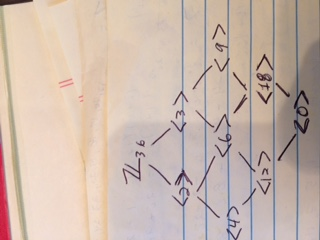
\includegraphics{IMG_2804}\\

25) Find the orders of all subgroups of $\mathbb{Z}_6$. \\

(Answer) : The subgroups of $\mathbb{Z}_6$ are
$$\langle 0 \rangle = \{0\}\;,$$
$$\langle 1 \rangle = \langle 5 \rangle = \{0,1,2,3,4,5\} \;,$$
$$\langle 2 \rangle = \langle 4 \rangle = \{0,2,4\}\;,$$
$$\langle 3 \rangle = \{0,3\} \;.$$
So we conclude that the orders of all subgroups of $\mathbb{Z}_6$ are 1,2,3,6. Note that when viewed as integers (instead of elements of $\mathbb{Z}_6$ which is unclear since we are being somewhat careless with notation for convenience), these are the positive divisors of 6. \\

39) The generators of the cyclic multiplicative group $U_n$ are the {\bf primitive $n^{th}$ roots of unity}. Find the primitive $n^{th}$ roots of unit when $n = 6$. \\

(Answer) : Recall $$U_6 = \{z \in \mathbb{C} | z^6 = 1\} = \{cos \left(\frac{2m\pi}{6} \right) + i\, sin \left(\frac{2m\pi}{6} \right) | m= 0,1,...5 \}$$
Note that $\langle e^{\frac{i\pi}{3}}\rangle = U_6$. Let $a = e^{\frac{i\pi}{3}}$. Suppose $b = a^s \in U_6$. Using Theorem 6.10, we know that $b$ generates $U_6$ as well if $gcd(s,6) = 1$. So $s = 1,5$. We have already given the result for $s = 1$ and $s = 5$ gives $e^{\frac{5 i \pi}{3}}$. Using Euler's formula and evaluating we conclude that the primitive 6th roots of unity are : $$\frac{1}{2} \pm \frac{\sqrt{3}}{2} i \;.$$

\subsection{Generating Sets and Cayley Digraphs}

\noindent \underline{\bf 7.4 Theorem} The intersection of some subgroups $H_i$ of a group $G$ for $i \in I$, (where $I$ is a collection of indices) is again a subgroup of $G$. \\

\noindent \underline{\bf 7.5 Definition} Let $G$ be a group and let $a_i \in G$ for $i \in I$. The smallest subgroup of $G$ containing $\{a_i \; | \; i \in I\}$ is the {\bf subgroup generated by} $\{a_i \; | \; i \in I \}$. If this subgroup is all of $G$, then $\{a_i \; | \; i \in I \}$ generates $G$ and the $a_i$ are {\bf generators of} $G$. If there is a finite set $\{a_i \; | \; i \in I \}$ that generates $G$, we say that $G$ is {\bf finitely generated}. \\

A note about this definition is that if an element of a set is part of set of elements that generate $G$, we call that element a generator even if that element by itself does not generate $G$. For example, $\{2,3\}$ generate $\mathbb{Z}_6$ since 2+3 = 5 and $\langle 5 \rangle = \mathbb{Z}_6$, so 2 and 3 are generators even though $\langle 2 \rangle \neq \mathbb{Z}_6$ and also $\langle 3 \rangle \neq \mathbb{Z}_6$. We should try to make it clear through context what exactly we mean in the future. \\

\noindent \underline{\bf 7.6 Theorem} If $G$ is a group and $a_i \in G$ for $i \in I$, then the subgroup $H$ of $G$ generated by $\{a_i \; | \; i \in I\}$ has as elements precisely those elements of $G$ that are finite products of integral powers of the $a_i$, where powers of a fixed $a_i$ may occur several times in the product. \\

\noindent \underline{\bf Notable Exercises} \\

1) List the elements generated by the subgroup $\{2,3\}$ of $\mathbb{Z}_12$. \\

(Answer) : Since $2 +_{12} 3 = 5$, and $gcd(5,12) = 1$, we know that $\{2,3\}$ generates $\mathbb{Z}_12$. Also it is not too difficult to find the integer linear combinations of 2,3 that do so, which was done on paper. \\

3) List the elements generated by the subgroup $\{8,10\}$ of $\mathbb{Z}_18$. \\

(Answer) : One approach is to find that $gcd(8,10) = 2$, and conclude the elements generated by this subgroup are numbers that 2 divides (up to class representatives), namely : $\{0,2,4,6,...,14,16\}$. \\

5) List the elements generated by the subgroup $\{12,42\}$ of $\mathbb{Z}$. \\

(Answer) : Using similar reasoning to before, and finding that $gcd(12,42) = 6$, we conclude the elements of $\mathbb{Z}$ generated by $\{12,42\}$ is : $\{0,\pm 6, \pm 12, \pm 18, .... \}$. \\

{\bf Remark :} I also found exercises 7, 9, 15, and 17 interesting / instructive but these rely on diagrams and tables from the book or hand drawn by the reader and so although they were worth working out, it is too time consuming to recreate the results in Latex.

\end{document}